

\documentclass[pdf]{beamer}
\usepackage{graphicx}
\usepackage{pgf}
\usepackage{tikz}
\usetikzlibrary{arrows,shapes}
\usepackage{verbatim}
\usetheme{Boadilla}
\setbeamertemplate{navigation symbols}{}

\title[Control rule evaluation]{
Quantifying the efficiency of harvest control rules in data limited situations
	}
\subtitle{
	}
\author[CE \& FS]{
	Charles T T Edwards and Finlay Scott
	}
\institute[IC London]{
	Imperial College London
	}
\date{May 2012}

\begin{document}



\frame{\titlepage}

\section{Overview}
\begin{frame}
\frametitle{Introduction}


\end{frame}

\section{Efficiency}

\begin{frame}
\frametitle{Efficiency}
The efficiency of estimation reflects ability of the harvest control rule to match the catch that would be expected with perfect knowledge of the resource

\begin{equation}
e(T) \propto \frac{1}{E[(\theta - \hat{\theta})^2]} \nonumber
\end{equation}
\end{frame}

\section{Data uncertainty}

\begin{frame}
\frametitle{Data uncertainty}
\framesubtitle{Observation error}

\begin{figure}
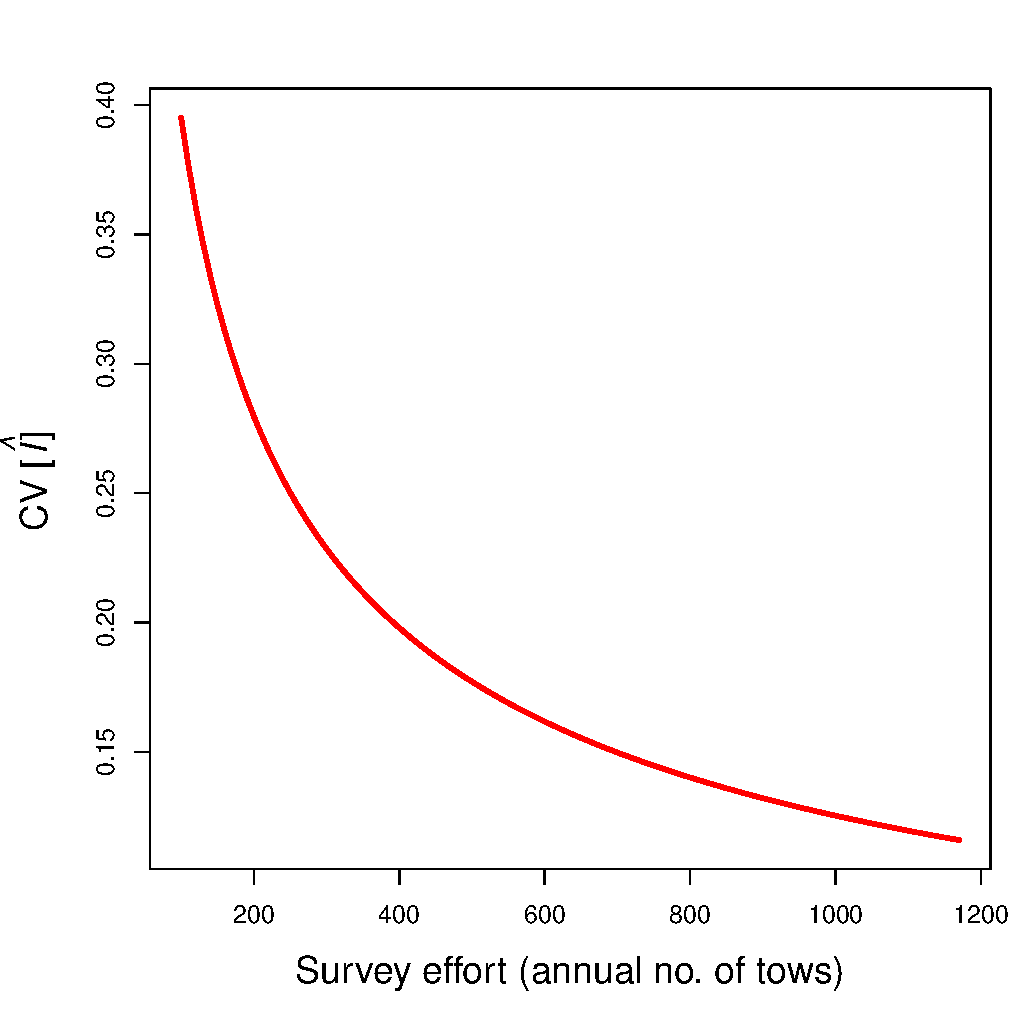
\includegraphics[width=0.6\textwidth]{../dat/obserror.pdf}
\end{figure}

\end{frame}

\begin{frame}
\frametitle{Data uncertainty}
\framesubtitle{Quantifying the information available to the control rule}
If $\varepsilon$ is the observation error residual, then the probability distribution of the mean residual is:
\begin{equation}
E[ln(\varepsilon)] \sim N\left(0,\sigma^2/n\right) \nonumber
\end{equation}
from which we obtain our measure of data uncertainty:
\begin{equation}
u(D) := \frac{\sigma}{\sqrt{n}} \nonumber
\end{equation}
where $n$ is the number of years of observation.
\end{frame}

\begin{frame}
\frametitle{Data uncertainty}
\framesubtitle{Simulation framework}

By changing the years of data available to the control rule ($n$) and the observation error ($\sigma$) we can modify the data uncertainty.

\begin{figure}
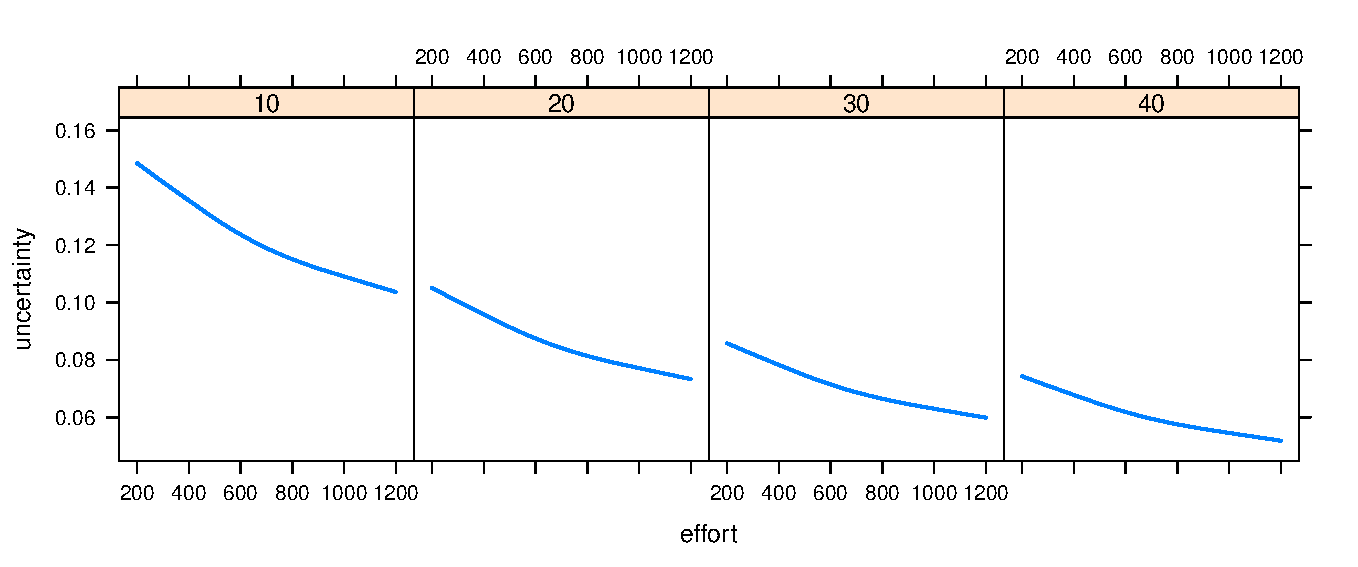
\includegraphics[width=1\textwidth]{../res/uncertainty.pdf}
\end{figure}

\end{frame}

\section{Simulations}
\begin{frame}
\frametitle{Experimental design}

We tested efficiency of the harvest conrol rule:
\begin{equation}
C_{y+1} = \frac{\hat{I}_{y+1}C^{TAR}}{I^{TAR}}\nonumber
\end{equation}

with four methods used to predict $\hat{I}_{y+1}$:
\begin{itemize}
\item Moving average
\item Linear regression
\item Smoothed index
\item Model based (Stock reduction analysis)
\end{itemize}

Simulations were repeated over a range of values for $n$ and $\sigma$.

\end{frame}

\begin{frame}
\frametitle{Simulation results}
\framesubtitle{Illustrative results}

\begin{figure}
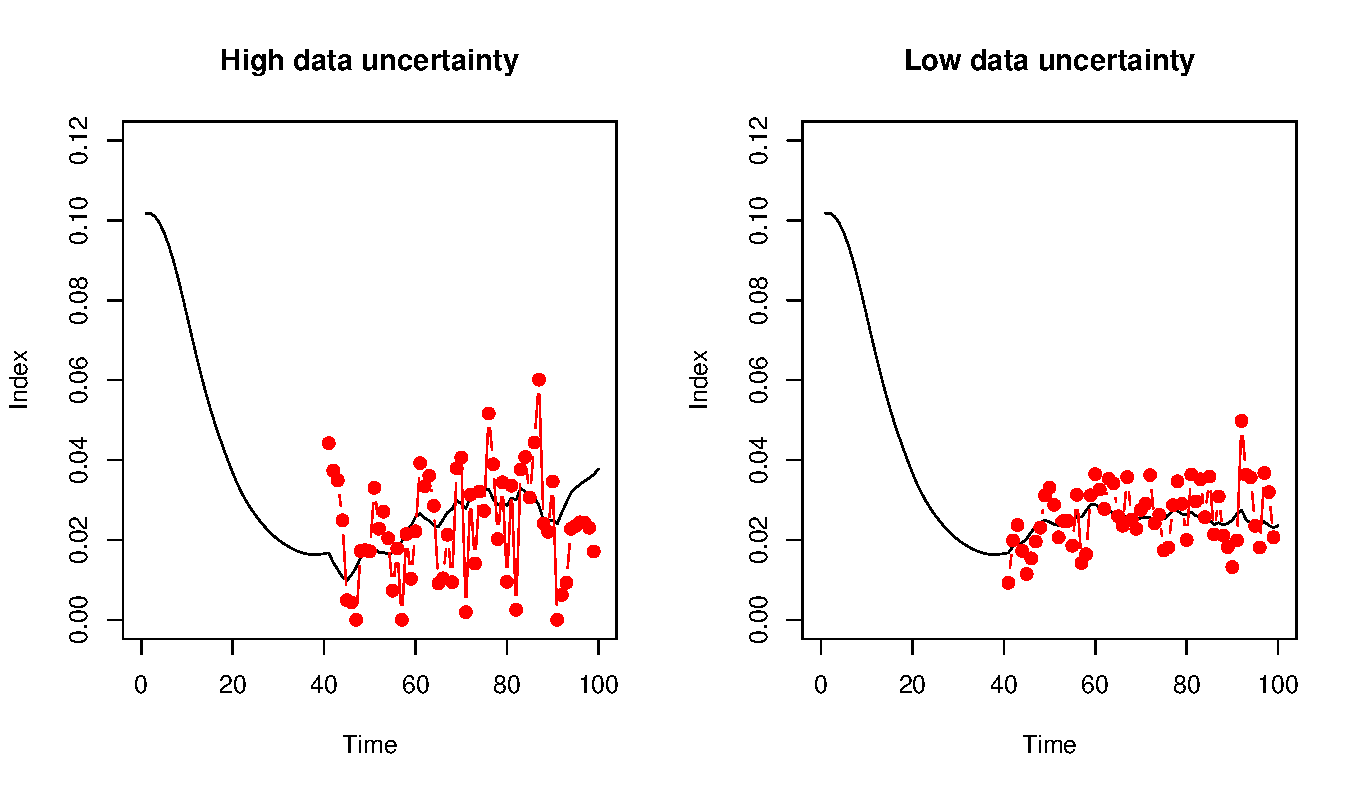
\includegraphics[width=0.9\textwidth]{../res/uncertainty_index.pdf}
\end{figure}

\end{frame}


\begin{frame}
\frametitle{Simulation results}
\framesubtitle{Combined results}

\begin{figure}
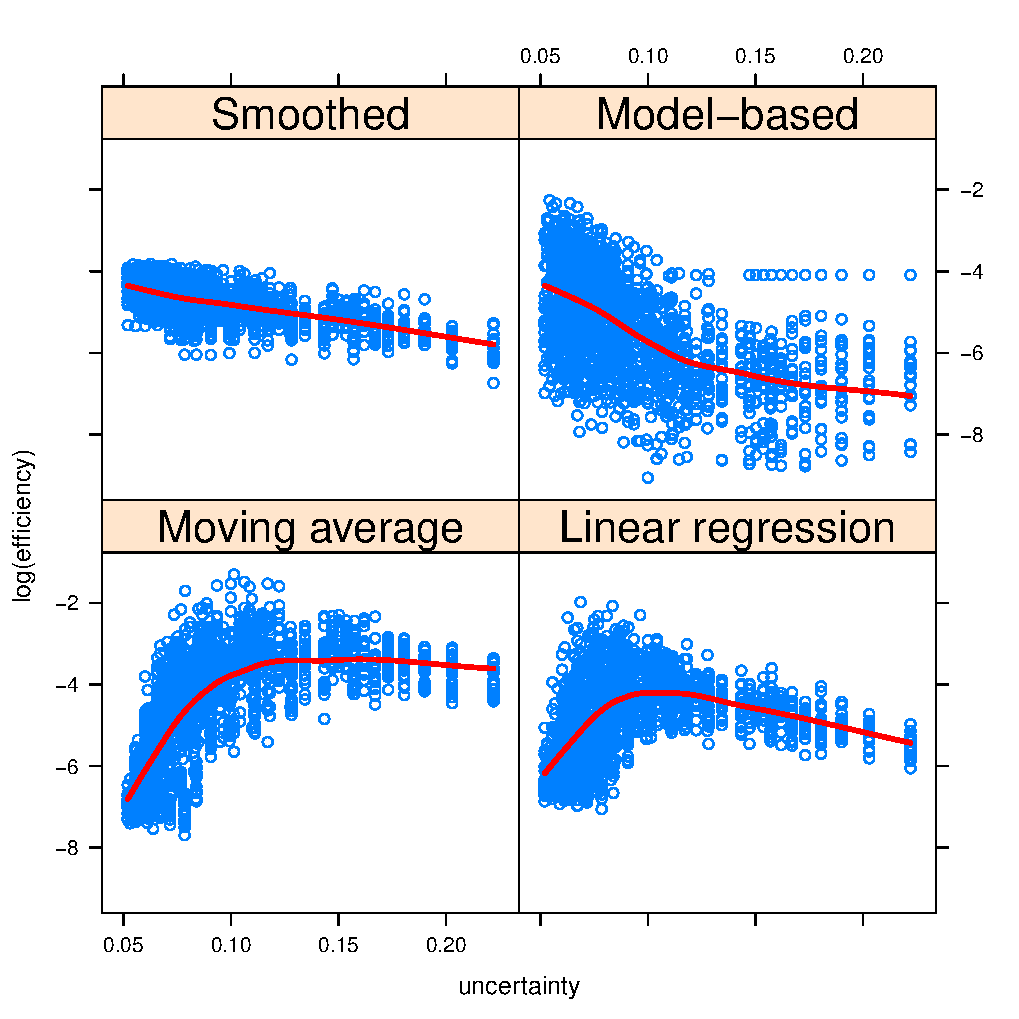
\includegraphics[width=0.6\textwidth]{../res/hcr_all_plot.pdf}
\end{figure}


\end{frame}


\end{document}
